\documentclass{article}
\title{\Huge Transform Techniques \& PDE}
\Large{\author{$\mathcal{WAFFLE'S\ \ CRAZY\ \ PEANUT}$}}
\date{(Last updated: 11/2/14)}
\usepackage{enumerate}
\usepackage{tikz}
\usepackage{tikz-qtree}
\usetikzlibrary{trees}
\usepackage{amsmath}
\newcommand{\para}[1]{\paragraph{#1}\mbox{}\\}
\usetikzlibrary{decorations.pathreplacing}
\pagenumbering{gobble}
\begin{document}
\maketitle
\textbf{\section{\huge Partial Differential Equations}}
\
{\Large 
\subsection{\LARGE Formation of PDE}
\paragraph{\Large Notations used:}
{\LARGE $$p=\frac{\partial \textbf{z}}{\partial x},\  q=\frac{\partial \textbf{z}}{\partial y}$$
$$r=\frac{\partial ^2\textbf{z}}{\partial x^2},\  s=\frac{\partial ^2\textbf{z}}{\partial x\partial y},\ t=\frac{\partial ^2\textbf{z}}{\partial y^2}$$}
\paragraph{\Large Type I: Elimination of arbitrary constants}
\begin{itemize}
\item If the number of arbitrary constants $=$ number of independent variables, first order PDE is enough.
\item If the number of arbitrary constants $>$ number of independent variables, higher orders are possible.
\end{itemize}
\newpage
\paragraph{\Large Type II: Elimination of arbitrary functions}
{\LARGE $$nf(x)=\mathcal{O}(PDE)$$}
\begin{center}
Number of functions $=$ Order of PDE
\end{center}
\
\paragraph{\Large Procedure:}
\begin{enumerate}[(a)]
\item Find the order of the required PDE by the number of arbitrary constants and independent variables (or) by the number of arbitrary functions.
\item Differentiate the function partially with respect to the independent variables to find the value of the arbitrary constants (or) arbitrary functions.
\item Replace the values with the exact notations.
\item Substitute in the given equation.
\newline
\end{enumerate}
\textbf{Note:} The goal is just to find a PDE for the given equation, by eliminating the arbitrary constants (or) arbitrary functions. If substitution doesn't work out, relate the different values from (b), to find the required PDE.
\newpage
\para{\Large Type III: Eliminating composite functions}
\
If the equation is of the form {\LARGE $F\big(u(x,y),v(x,y)\big)=0$}, the direct solution is,
{\LARGE $$pP+qQ=R$$
$$P=\begin{vmatrix}
u_y & v_y  \\
u_z & v_z  \\
\end{vmatrix}\ \ 
Q=\begin{vmatrix}
u_x & v_x  \\
u_z & v_z  \\
\end{vmatrix}$$
$$R=\begin{vmatrix}
u_x & v_x  \\
u_y & v_y  \\
\end{vmatrix}$$}
\newline
\subsection{\LARGE Solutions of PDE}
A solution can either be made of arbitrary constants or arbitrary functions. Both are valid for the same PDE.
\newline
\begin{center}
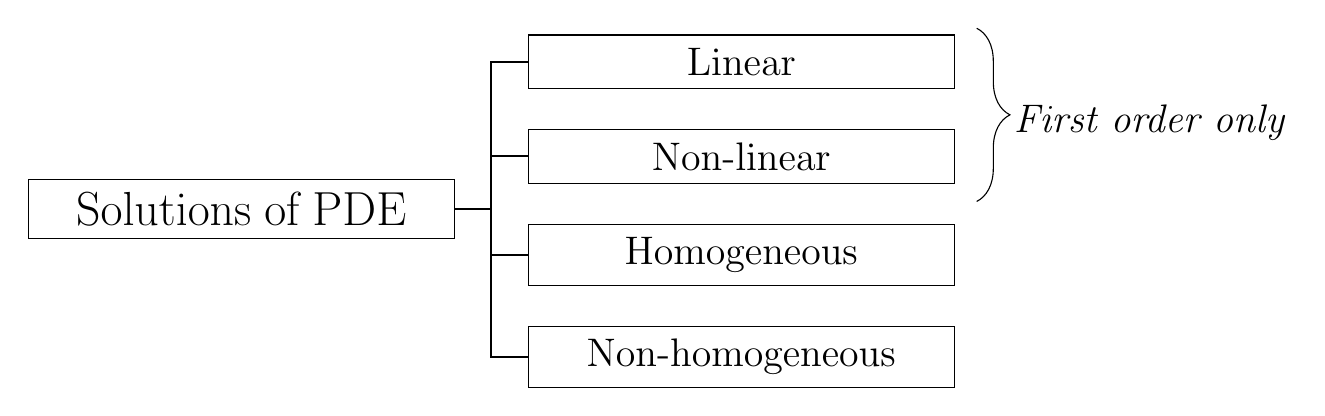
\begin{tikzpicture}[grow'=right,level distance=2.5in,sibling distance=.2in]
\tikzset{edge from parent/.style= 
            {thick, draw, edge from parent fork right},
         every tree node/.style=
            {draw,minimum width=2in,text width=2in,align=center}}
{\Large \Tree 
    [. {{\LARGE Solutions of PDE}}
        [.Linear ]
        [.Non-linear ]
        [.Homogeneous ]
        [.Non-homogeneous ]
    ]}
\draw [decorate,decoration={brace,amplitude=12pt,mirror,raise=4pt},yshift=0pt]
    (9.2,0.1) -- (9.2,2.3) node [black,midway,xshift=2.35cm,yshift=-0.1cm] {\footnotesize
    {\Large \textit{First order only}}};
\end{tikzpicture}
\end{center}
\newpage
\para{\LARGE Linear PDE:}
\\
Characteristics:
\begin{itemize}
\item It is of the \textbf{first} degree.
\item It has no products of the dependent variable.
\item Power of its dependent variable should be \textbf{1}.
\end{itemize}
$\ $
\para{\Large Type I: Direct Method}
The solution is obtained by directly integrating the respective PDEs. For e.g. (using notations $q,s$),
\\
{\LARGE $$s=\frac{x}y$$
$$q=\int s\cdot dx=\frac{x^2}{2y}+f(y)$$
$$\int q\cdot dy=\frac{x^2}2\ log_e(y)+\int f(y)\cdot dy+g(x)$$
$$\implies\mathbf{z}=\frac{x^2}2\ log_e(y)+\phi(y)+g(x)$$}
\newpage
\paragraph{{\Large Note:}}
\begin{enumerate}[(a)]
\item In this method, you can begin your integration by using any of the independent variables (i.e) $x$ or $y$. That's because most of our problems treat PDEs to be homogeneous.
$\\ $
\item $\mathbf z$ is a $f(x,y)$. When you integrate $\mathbf z$ with respect to $x$, the integration constant could be a function of $y$. So, the constants that come out during integration, should be replaced by new functions $f(y)$, $g(x)$, etc.
$\\ $
\item $\phi(y)$ denotes that you've already integrated $f(y)$, and it should be distinguished from its parent - $\phi(y)$. And, $g(x)$ has appeared as a result of integrating $f(y)$ due to the same reason mentioned at (b).
$\\ $
\item Cases where the function itself depends on its own derivative, such as $\textbf{z}=t$ \textit{(notation)}, can be solved by using a characteristic function (same as in ODE), which includes all possible constants (so, you don't have to insert a constant after each integration).

Just integrate, find the values of the functions, and substitute in C.F.
\end{enumerate}
\newpage
\para{\Large Type II: Lagrange's method for Quasi-linear PDE:}
In such PDEs, the highest order derivatives are linear, with coefficients existing as a function of lower order derivatives of dependent variables. \begin{center}
{\LARGE $\textbf{z}xp+\textbf{z}yq=\textbf{z}xy\ $} is an example.
\end{center}
\paragraph{\Large Procedure:}
\begin{enumerate}[(a)]
\item Check whether the PDE is of first degree.
\item Given equation should be of the quasi-linear form {\Large $pP+qQ=R$}. If it's not, then make it!
\item Substitute in the equation,
{\LARGE $$\frac{dx}{P}=\frac{dy}{Q}=\frac{dz}{R}$$} \\
Rearrange the equation (variable-separable method) i.e., $x$ terms to the side of $dx$, $y$ terms to $dy$, etc., and integrate them. \\

\textbf{Note:} Independent variables should never be treated as constants during this integration. For e.g., you cannot have a $y$ term along with the $x$ terms as a product, and treat them as a constant during the integration with respect to $x$.
\item Find ``two solutions" by equating any two of the equations (any way), and integrating them as a whole.
\item Substitute the constants obtained from integration (which are a function of the independent variables) into the equation,
$$F(C_1,C_2)=0$$
\textbf{Note:} Both the solutions should be independent of each other. For e.g., $C_1=3C_2$ is not a valid solution.
\end{enumerate}
$\ $
\paragraph{\Large If it fails at (c):} Some composite functions cannot be eliminated by variable-separable method, when you
\begin{enumerate}[(i)]
\item Choose three constants $l$, $m$ and $n$, such that {\LARGE $$lP+mQ+nR=0$$}
\item Substitute $l$, $m$ and $n$ in the equation, and integrate with respect to the independent variables, to obtain an expression (say, $U$). {\LARGE $$\int l\cdot dx+\int m\cdot dy+\int n\cdot dz=0$$}
\item Now, use another set of unique values for $l$, $m$ and $n$ satisfying (i), and follow the same steps to obtain another expression (say $V$).
\item Substitute in the equation,
{\LARGE $$F(u,v)=0$$}
\end{enumerate}
\newpage
\subsection{\LARGE Non-linear PDE:}
Characteristics:
\begin{itemize}
\item Degree higher than 1.
\item Product of $p$ and $q$, or with the dependent variable.
\end{itemize}
$\ $
\paragraph{\LARGE Procedure for solving different types:}
\para{{\Large \underline{Type 1}: {\LARGE $\ F(p,q)=0$}}}
\begin{itemize}
\item Complete solution:
\begin{enumerate}[1)]
\item Write complete solution: {\LARGE $$\textbf{z}=ax+by+c$$}
\item Substitute $(a,b)$ for $(p,q)$ in the given function, and find {\LARGE $b=f(a)$} by equating {\LARGE $f(a,b)=0$}.
\item Substitute {\LARGE $b=f(a)$} in the complete solution,{\LARGE $$\textbf{z}=ax+f(a)y+c$$}.
\end{enumerate}
\item General solution:
\begin{enumerate}[1)]
\item Substitute {\LARGE $c=\phi(a)$} in the complete solution, {\LARGE $$\textbf{z}=ax+f(a)y+\phi(a)$$}.
\item Differentiate partially with respect to $a$, {\LARGE $$x+f'(a)y+\phi'(a)=0$$}.
\item \textbf{Don't forget} to write, ``By eliminating {\LARGE $a$} from (1) and (2), we obtain the general solution".
\end{enumerate}
$\ $
\item Singular solution: \\
Partially differentiate complete solution with respect to {\LARGE $c$}, and you'll get {\LARGE $0=1$}. But since {\LARGE $0\neq 1$}, there's \textbf{no singular solution}.
\end{itemize}
\para{{\Large \underline{Type 2}: {\LARGE $\ F(\textbf{z},p,q)=0$}}}
\begin{itemize}
\item Complete solution:
\begin{enumerate}[1)]
\item Let {\LARGE $u=x+ay$
$$\frac{\partial u}{\partial x}=1,\  \frac{\partial u}{\partial y}=a$$}
Since {\LARGE $u=f(x,y)$}, {\LARGE $\textbf{z}$} can be {\LARGE $f(u)$}.
{\LARGE $$\implies p=\frac{\partial \textbf{z}}{\partial x}=\frac{d \textbf{z}}{d u}\cdot\frac{\partial u}{\partial x}=\frac{d \textbf{z}}{d u}$$}
{\LARGE $$\implies q=\frac{\partial \textbf{z}}{\partial y}=\frac{d \textbf{z}}{d u}\cdot\frac{\partial u}{\partial y}=a\frac{d \textbf{z}}{d u}$$}
\newpage
\item Substitute the ``new" $p,q$ in {\LARGE $F(\textbf{z},p,q)=0$}.
\item Rearrange the equation (variable-separable method), and integrate it with the respective $(u,\textbf{z})$, to get the corresponding $f(u,\textbf{z})$.
\item Substitute {\LARGE $u=x+ay$} in the equation, and rearrange it, to obtain the complete solution in the form {\LARGE $\textbf{z}=f(x,y)\\ $}.
\end{enumerate}
\item General solution:
\begin{enumerate}[1)]
\item Substitute {\LARGE $c=\phi(a)$} in the complete solution.
\item Differentiate partially with respect to $a$.
\item \textbf{Don't forget} to write, ``By eliminating {\LARGE $a$} from expressions (1) and (2), we obtain the general solution".
\end{enumerate}
$\ $
\item Singular solution: \\
Partially differentiate complete solution with respect to {\LARGE $c$}, and you'll get {\LARGE $0=1$}. But since {\LARGE $0\neq 1$}, there's \textbf{no singular solution}.
\end{itemize}
\para{{\Large \underline{Type 3}: {\LARGE $\ F(x,p)=f(y,q)$}}}
\begin{itemize}
\item Complete solution:
\begin{enumerate}[1)]
\item Rearrange the expression to the required form, and equate the functions to constant {\LARGE $a$}, {\LARGE $$F(x,p)=f(y,q)=a$$}
\item Obtain $(p,q)$ from the above as, {\LARGE $$p=\phi(x,a),\ q=\psi(y,a)$$}
\item Substitute $(p,q)$ in the equation $d\textbf{z}=pdx+qdy$, and integrate it to get $\textbf{z}$. {\LARGE $$\int d\textbf{z}=\int p\cdot dx+\int q\cdot dy$$}
\end{enumerate}
\item General solution:
\begin{enumerate}[1)]
\item Substitute {\LARGE $c=\phi(a)$} in the complete solution.
\item Differentiate partially with respect to $a$.
\item \textbf{Don't forget} to write, ``By eliminating {\LARGE $a$} from expressions (1) and (2), we obtain the general solution".
\end{enumerate}
$\ $
\item Singular solution: \\
Partially differentiate complete solution with respect to {\LARGE $c$}, and you'll get {\LARGE $0=1$}. But since {\LARGE $0\neq 1$}, there's \textbf{no singular solution}.
\end{itemize}
\para{{\Large \underline{Type 4}: {\LARGE $\ \textbf{z}=px+qy+f(p,q)$}}}
\begin{itemize}
\item Complete solution: \\
Substitute {\LARGE $p=a$}, {\LARGE $q=b$} in the given equation to get the complete solution, {\LARGE $$\textbf{z}=ax+by+f(a,b)$$}
\newpage
\item General solution:
\begin{enumerate}[1)]
\item Substitute {\LARGE $b=\phi(a)$} in the complete solution, {\LARGE $$\textbf{z}=ax+\phi(a)y+f\big(a,\phi(a)\big)$$}
\item Differentiate partially with respect to $a$, {\LARGE $$x+\phi'(a)y+f'\big(a,\phi(a)\big)=0$$}
\item \textbf{Don't forget} to write, ``By eliminating {\LARGE $a$} from expressions (1) and (2), we obtain the general solution".
\end{enumerate}
\item Singular solution: (Type 4 \textit{has} singular solution)
\begin{enumerate}[1)]
\item Partially differentiate complete solution with respect to {\LARGE $(a,b)$}, to obtain two equations.
\item Do any substitution possible, to eliminate the constants, and arrive at a generalized solution, as singular solution doesn't have constants!
\end{enumerate}
\end{itemize}
\paragraph{\Large Reduction to Standard form:}
\begin{itemize}
\item For equations of the form {\LARGE $F(x^m\textbf{z}^kp,y^n\textbf{z}^kq)=0$}, substitute
{\LARGE $$X=\begin{cases}
x^{1-m},\ m\neq 1\\
log(x),\ m=1
\end{cases} Y=\begin{cases}
y^{1-n},\ n\neq 1\\
log(y),\ n=1
\end{cases}$$ $$\textbf{Z}=\begin{cases}
\textbf{z}^{k+1},\ k\neq -1\\
log(\textbf{z}),\ k=1
\end{cases}$$}
\item Updated notations are,
{\LARGE $$P=\frac{\partial \textbf{Z}}{\partial X}=\frac{\partial \textbf{Z}}{\partial \textbf{z}}\cdot\frac{\partial \textbf{z}}{\partial x}\cdot \frac{\partial x}{\partial X}$$ $$Q=\frac{\partial \textbf{Z}}{\partial Y}=\frac{\partial \textbf{Z}}{\partial \textbf{z}}\cdot\frac{\partial \textbf{z}}{\partial y}\cdot \frac{\partial y}{\partial Y}$$}
\item Substitute $P$ and $Q$ in the given equation, and solve the non-linear PDE, by finding the type.
\end{itemize}
\textbf{Note:} For the complete, general, and singular solutions, don't forget to replug the original $x,y,p,q$.
\subsection{\LARGE Solving linear homogeneous n$\mathrm{^{\textbf{th}}}$ order PDE with constant coefficients:}
Equation of the form, ({\LARGE $a_0,a_1,a_2,...\ a_n=$} constants)
{\LARGE $$a_0\frac{\partial^n \textbf{z}}{\partial x^n}+a_1\frac{\partial^n \textbf{z}}{\partial x^{n-1}\partial y}+a_2\frac{\partial^n \textbf{z}}{\partial x^{n-2}\partial^2 y}+...\ +a_n\frac{\partial^n \textbf{z}}{\partial y}=f(x,y)$$}
Solution is $\textbf{z}=\mathrm{C.F+P.I}$
\paragraph{{\Large Characteristic function:}}
\begin{enumerate}[(i)]
\item Express in symbolic form,
{\LARGE $$D=\frac{\partial}{\partial x},\ D'=\frac{\partial}{\partial y}$$}
\item Put $D'=1$, $D=m$, and equate {\LARGE $f(m)=0$}, to find the roots $m_1$ and $m_2$.
\newpage
\begin{itemize}
\item For real and distinct roots, {\LARGE $$\mathrm{C.F}=f_1(y+m_1x)+f_2(y+m_2x)$$}
\item For real and equal roots, {\LARGE $$\mathrm{C.F}=f_1(y+mx)+xf_2(y+mx)$$}
\end{itemize}
\end{enumerate}
\paragraph{{\Large Particular Integral:} {\LARGE $$\mathrm{P.I}=\frac{F(x,y)}{f(D,D')}$$}}
\begin{itemize}
\item {\LARGE $F(x,y)=e^{ax+by}$}
{\LARGE $$D=a,\ D'=b$$ $$\mathrm{P.I}=e^{ax+by}\cdot \frac{1}{f(a,b)}$$} \\
\item {\LARGE $F(x,y)=\mathrm{sin}(ax+by)$} or {\LARGE $\mathrm{cos}(ax+by)$}
{\LARGE $$D^2=-a^2,\ D'^2=-b^2,\ DD'=-ab$$ $$\mathrm{P.I}=F(x,y)\cdot \frac{1}{f(-a^2,-ab,-b^2)}$$} \newpage
\item {\LARGE $F(x,y)=x^my^n$}
\begin{enumerate}[1)]
\item Take a higher-order term out of the denominator, and bring the remaining up! (inverse),
{\LARGE $$\mathrm{P.I}=\frac{F(x,y)}{1+f(D,D')}$$ $$\implies\mathrm{P.I}=(1+f(D,D'))^{-1}\cdot F(x,y)$$}
\item Expand using binomial expansion (stopping with PDE's highest order as $n$, which is mostly `2'), $$(1+x)^{-1}=1-x+x^2$$
\item Multiply the expressions, and differentiate $F(x,y)$ if it's $D$, and integrate if it's {\LARGE $1\over D$}\\
\end{enumerate}
\item {\LARGE $F(x,y)=\phi(x,y)$}
\begin{enumerate}[1)]
\item Factorize the denominator as $(D,m_1D')(D,m_2D')$
\item Substitute {\LARGE $y=c-m_1x$} in the numerator, and integrate it with respect to {\LARGE $x$}, while neglecting $(D,m_1D')$ in the denominator.
\item Loop (2), until the denominator vanishes.
\end{enumerate}
For e.g., {\LARGE $$\mathrm{P.I}=\frac{(y-1)e^x}{D^2-DD'-2D'^2}$$}
\newpage
{\LARGE $$=\frac{(y-1)e^x}{(D-2D')(D+D')}\\ $$} Sub. {\LARGE $y=c-2x$, $$=\frac{1}{D+D'}\int(c-2x-1)e^x\cdot dx$$ $$=\frac{1}{D+D'}(y+1)e^x\\ $$} Sub. {\LARGE $y=c+x$, $$=\int(c+x+1)e^x\cdot dx\ =ye^x$$}
\end{itemize}
\subsection{\LARGE Solving linear non-homogeneous n$\mathrm{^{\textbf{th}}}$ order PDE with constant coefficients:}
\begin{enumerate}[(i)]
\item Factorize the mixture of $D,D',D^2,D'^2,DD'$ to one of the forms,
\begin{itemize}
\item {\LARGE $(D-m_1D'-c_1)(D-m_2D'-c_2)$}
\item {\LARGE $(D'-m_1D-c_1)(D'-m_2D-c_2)$}
\end{itemize}
\item Find the coefficients {\LARGE $m$} and {\LARGE $c$}.
\item Substitute in the respective C.F,
\begin{itemize}
\item {\LARGE $e^{c_1x}f_1(y+mx)+e^{c_2x}f_2(y+mx)$}
\item {\LARGE $e^{c_1y}f_1(x+my)+e^{c_2y}f_2(x+my)$}
\end{itemize}
\item Finding P.I remains the same.
\end{enumerate}
\subsection{\LARGE Second-order PDE:}
General form: {\LARGE $$\big(AD^2+BDD'+CD'^2\big)\textbf{z}=F(x,y)$$} where $A$, $B$, $C$ are $f(x,y)$
\begin{itemize}
\item $B^2-4AC<0\to$ elliptic
\item $B^2-4AC=0\to$ parabolic
\item $B^2-4AC>0\to$ hyperbolic
\end{itemize}
$\ $
\subsection{\LARGE Integral surface passing through the given curve:}
\paragraph{\Large Procedure:}
\begin{enumerate}[(i)]
\item Solve the PDE by \textit{any} method (pg. no. 8 $\to$ 16)
\item Substitute the solutions in the given curves, and relate them in any way to get the ``constant-less" general equation (similar to singular solution).
\end{enumerate}
This equation gives a curve that passes through both of the given curves.
\newpage
\textbf{\section{\huge Fourier Series}}
$\ $
\subsection{{\LARGE Dirichlet's Condition:}}
The given function $f(x)$
\begin{itemize}
\item is finite, periodic, single-valued
\item has finite number of discontinuities
\item has the utmost finite number of maximas \& minimas
\end{itemize}
$\ $
\subsection{\LARGE General Fourier Series:}
For a periodic function defined over {\LARGE $(c,c+2l)$},
{\LARGE $$f(x)=\frac{a_0}{2}+\sum_{n=1}^\infty a_n\ \mathrm{cos}\bigg(\frac{n\pi x}{l}\bigg)+\sum_{n=1}^\infty b_n\ \mathrm{sin}\bigg(\frac{n\pi x}{l}\bigg)$$}
where {\LARGE $a_0$}, {\LARGE $a_n$} \& {\LARGE $b_n$} are Euler's integrals
{\LARGE $$a_0=\frac{1}l\int_c^{c+2l} f(x)\cdot dx$$
$$a_n=\frac{1}l\int_c^{c+2l} f(x)\cdot \mathrm{cos}\bigg(\frac{n\pi x}{l}\bigg)\cdot dx$$
$$b_n=\frac{1}l\int_c^{c+2l} f(x)\cdot \mathrm{sin}\bigg(\frac{n\pi x}{l}\bigg)\cdot dx$$}
$\ $
If the given interval is of the form {\LARGE {\LARGE $(-l,l)$}} - either as a whole (or) split into multiple intervals for defining a discontinuous function, check whether the function is odd or even.
\\
\\
\textbf{Note:} For discontinuous functions, be sure to switch the inequalities when `minus' sign is encountered.
\para{\Large Case 1: Odd function {\LARGE $f(-x)\neq f(x)$}}
{\LARGE $$a_0=0,\ a_n=0$$
$$b_n=\frac{2}l\int_0^lf(x)\cdot \mathrm{sin}\bigg(\frac{n\pi x}{l}\bigg)\cdot dx$$
$$\implies f(x)=\sum_{n=1}^\infty b_n\ \mathrm{sin}\bigg(\frac{n\pi x}{l}\bigg)$$}
\para{\Large Case 2: Even function {\LARGE $f(-x)=f(x)$}}
{\LARGE $$a_0=\frac{2}l\int_0^l f(x)\cdot dx$$
$$a_n=\frac{2}l\int_0^l f(x)\cdot \mathrm{cos}\bigg(\frac{n\pi x}{l}\bigg)\cdot dx$$
$$b_n=0$$
$$\implies f(x)=\frac{a_0}2+\sum_{n=1}^\infty a_n\ \mathrm{cos}\bigg(\frac{n\pi x}{l}\bigg)$$}
\paragraph{\Large Case 3: Neither odd, nor even}
\begin{center}
{\LARGE $f(x)$} remains the same
\end{center}
$\ $
\subsection{\LARGE Convergence:}
If the given {\LARGE $f(x)$} converges at {\LARGE $x=\alpha$},
\begin{itemize}
\item which is a limit of the given function, then {\LARGE $$f(x)=\frac{1}2\big[f(c)+f(c+2l)\big]$$}
\item which is a discontinuity, then
{\LARGE $$f(x)=\frac{1}2\big[f(x^-)+f(x^+)\big]$$}
\item and, if it's continuous, then {\LARGE $f(x)=\alpha$}.
\end{itemize}
$\ $
\subsection{\LARGE Half-range Expansion:}
{\LARGE $f(x)$} over the interval {\LARGE $(o,c)$} can be expanded into two distinct half-range series.
\begin{itemize}
\item \textbf{Half-range cosine series:}
{\LARGE $$f(x)=\frac{a_0}2+\sum_{n=1}^\infty a_n\ \mathrm{cos}\bigg(\frac{n\pi x}{l}\bigg)$$
$$a_0=\frac{2}l\int_0^c f(x)\cdot dx$$}
{\LARGE $$a_n=\frac{2}l\int_0^c f(x)\cdot \mathrm{sin}\bigg(\frac{n\pi x}{l}\bigg)\cdot dx$$}
$\ $
\item \textbf{Half-range sine series:}
{\LARGE $$f(x)=\sum_{n=1}^\infty b_n\ \mathrm{sin}\bigg(\frac{n\pi x}{l}\bigg)$$
$$b_n=\frac{2}l\int_0^c f(x)\cdot \mathrm{sin}\bigg(\frac{n\pi x}{l}\bigg)\cdot dx$$}
\end{itemize}
$\ $
\subsection{\LARGE Root Mean Square:}
{\LARGE $$[f(x)]_{\mathrm{rms}}=\sqrt{\frac{1}{b-a}\int_a^b f(x)^2\cdot dx}$$}
\subsection{\LARGE Passeval's Identity:}
If {\LARGE $f(x)$} has a Fourier series (i.e.) the function satisfies Dirichlet's condition, and has a period of {\LARGE $(-l,l)$}, then
{\LARGE $$\frac{1}l\int_{-l}^{l}\big(f(x)\big)^2\cdot dx=\frac{a_0^2}2+\sum_{n=1}^\infty(a_n^2+b_n^2)$$}
\newpage
\para{\Large Corollary:}
\begin{enumerate}[(i)]
\item If the interval is ${\LARGE (0,2l)}$ {\LARGE $$\int_{0}^{2l}\big(f(x)\big)^2\cdot dx=l\ \bigg(\frac{a_0^2}2+\sum_{n=1}^\infty(a_n^2+b_n^2)\bigg)$$}
\item For half-range cosine series,
{\LARGE $$\int_0^l\big(f(x)\big)^2\cdot dx=\frac{l}2\ \bigg(\frac{a_0^2}2+\sum_{n=1}^\infty a_n^2\bigg)$$}
\item For half-range sine series,
{\LARGE $$\int_0^l\big(f(x)\big)^2\cdot dx=\frac{l}2\ \bigg(\sum_{n=1}^\infty b_n^2\bigg)$$}
\end{enumerate}
$\ $
\subsection{\LARGE Complex form of Fourier series:}
$\ $
{\LARGE $$f(x)=\frac{a_0}2+\sum_{n=1}^\infty \frac{(a_n-i\ b_n)}2\ e^{i\frac{n\pi x}{l}}+\sum_{n=1}^\infty \frac{(a_n+i\ b_n)}{2i}\ e^{-i\frac{n\pi x}{l}}$$}
$$\mathrm{(OR)}$$
{\LARGE $$f(x)=C_0+\sum_{n=1}^\infty C_n\ e^{i\frac{n\pi x}{l}}+\sum_{n=1}^\infty C_{-n}\ e^{-i\frac{n\pi x}{l}}$$}
\newpage
{\LARGE $$C_n=\frac{(a_n-i\ b_n)}2$$ $$C_n=\frac{1}{2l}\int_{-l}^{l}f(x)\cdot e^{-i\frac{n\pi x}{l}}\cdot dx$$}
\\
For values of $n=0,1,\ \& -1$, corresponding values of $C_0,C_n,\ \&\ C_{-n}$ can be generated. So,
{\LARGE $$f(x)=\sum_{n=-\infty}^\infty\ C_n\ e^{i\frac{n\pi x}{l}}$$}
\subsection{\LARGE Harmonic Analysis: (numerical)}
{\LARGE $$\mathrm{Mean\ of\ } f(x)=\frac 1{b-a}\int_a^b f(x)\cdot dx$$}
{\LARGE $$\frac{a_0}2=\mathrm{Mean\ of\ } f(x) \implies a_0=\frac{2 \sum y}{N}$$}
{\LARGE $$a_n=\frac{2\sum y\cdot \mathrm{cos}\ (\frac{n\pi x}{l})}{N}$$}
{\LARGE $$b_n=\frac{2\sum y\cdot \mathrm{sin}\ (\frac{n\pi x}{l})}{N}$$}
\\
Tabulate the values, and write the summed up {\LARGE $f(x)$}, up to the $n$-values specified in the question.
\newpage
\textbf{\section{\huge Applications of PDE}}
$\ $
\subsection{\LARGE Solving Linear PDE:}
Most of the ``linear PDE" can be solved by using variable-separable method.
\paragraph{\Large Procedure:}
\begin{enumerate}[(a)]
\item Write the assumption {\LARGE $\textbf{Z}=X(x)\cdot Y(y)$}
\item Using the assumption, reformulate the given PDE in terms of $X$ and $Y$ (i.e.) substitute, and partially differentiate with respect to independent variables.
\item Separate $X$ and $Y$ terms, and equate them to some constant (say `{\LARGE $a$}').
\item Individually solve the ODE by integrating the terms along with {\LARGE $a$}.
\item Substitute the obtained $X$ and $Y$ in the assumption (a) to get the required function $\textbf{Z}$.
\end{enumerate}
\end{document}
